\section{矩阵低秩逼近}
\label{sec:ls-matrix-low-rank}
\label{sec:matrix-analysis-svd-low-rank}
\label{sec:ch06-rank-constrained-approximation}
\label{sec:ch06-error-constrained-rank}

第~\ref{sec:ls-least-squares}节在固定形状的输入向量中挑选系数，使输出残差最小；
本节改变任务对象：未知量本身是一张矩阵，要求它在保持主要作用的同时占用更少参数。
一张$m\times n$稠密矩阵需要存储$mn$个数，每次作用需要$O(mn)$次运算；推荐系统的评分
矩阵、一幅图像或一批样本的设计矩阵，$mn$轻易达到百万级，直接存储和运算都不现实。
这类矩阵的信息常高度集中：少数几个输入方向被放大后送入配对的输出方向，就解释了大部分
作用。自然的问题是：能否只保留最重要的$k$个方向，用远少于$mn$的参数近似整张矩阵？
若能以$k$个输入输出方向的配对近似它，存储和作用成本便可降到$O((m+n)k)$。

特征向量要求输出回到输入的同一方向，因而适合分析同一空间内的反复作用；压缩却要问哪些
输入方向的作用最值得保留，并允许输出落到另一个方向。三维输入送入二维输出时已经无法要求
两端沿同一条方向；又如把用户作为行、影片作为列，评分矩阵$\bm R\in\mathbb R^{n_{\mathrm u}\times n_{\mathrm m}}$
中$\bm v\mapsto\bm R\bm v$把影片坐标映到用户坐标，两端本就是不同对象的坐标，谈不上同一个
特征方向。因此本节使用第~\ref{sec:ls-svd}节已经建立的奇异值分解：定义域与陪域各自选取
正交方向，有非零作用的输入方向分别被缩放后送入配对的输出方向，其余方向映为零。
存在性与构造不再重复，本节只在这一工具上回答规模怎样度量、最优候选是谁、怎样计算与核验。

\subsection{目标与误差}
\label{sec:ls-low-rank-objective}

\paragraph{秩预算与误差范数}

先规定规模预算：给定整数$k$，在所有秩不超过$k$的矩阵中寻找离$\bm A$最近的候选
$\bm B$。误差口径先于方向选择确定，常用两种：谱范数误差
$\lVert\bm A-\bm B\rVert_2=\max_{\lVert\bm x\rVert_2=1}\lVert(\bm A-\bm B)\bm x\rVert_2$
度量任意单位输入的最坏输出偏差；Frobenius误差
$\lVert\bm A-\bm B\rVert_{\mathrm F}=(\sum_{i,j}(a_{i,j}-b_{i,j})^2)^{1/2}$
对一组标准输入方向的输出偏差平方求和后开方。两者回答不同问题：前者保证最坏方向不失真，
后者累计全部坐标的总偏差，不能互相替代。

由~\ref{thm:ls-svd-existence}，$\bm A\in\mathbb R^{m\times n}$有分解
$\bm A=\bm U\bm\Sigma\bm V^\top$，非零奇异值按降序记为
$\sigma_1\geq\cdots\geq\sigma_r>0$，$r=\operatorname{rank}\bm A$。
下面所有结论都以这一给定分解为输入，不再重新证明奇异值的存在性。

\paragraph{秩约束与核范数惩罚的区别}

固定秩约束$\operatorname{rank}\bm B\leq k$是一个硬预算：可行集合由若干低维线性流形
拼成，不是凸集，候选不能沿线段自由插值。另一条路线不在参数上设限，而在拟合目标中附加
对矩阵“大小”的凸惩罚：
\begin{equation}
 \min_{\bm B}\ \tfrac12\lVert\bm A-\bm B\rVert_{\mathrm F}^2
 +\lambda\lVert\bm B\rVert_*,
 \qquad \lambda\geq0,
 \label{eq:ls-nuclear-penalty-problem}
\end{equation}
其中$\lVert\cdot\rVert_*$是稍后定义的核范数。惩罚改变的是目标本身：$\lambda$越大，
保留下来的奇异尺度被压得越小，它产生的实际秩取决于原谱，不等于直接指定$k$。
硬预算回答“最多用$k$个方向能做到多好”，惩罚问题回答“拟合与简洁之间怎样折中”，
两者的最优解一般不同，求解路径也不同，不能不加说明地当成同一个截断问题。

\subsection{规模与误差的比较}
\label{sec:ls-rank-scale-comparison}

\subsubsection{秩与保留信息}
\label{sec:ls-rank-and-information}

\paragraph{精确非零方向与代数秩}

代数秩$r=\operatorname{rank}\bm A$是非零奇异值的个数，也就是$\bm A$真正使用的
精确非零方向数：$\bm A=\sum_{i=1}^r\sigma_i\bm u_i\bm v_i^\top$中每一项对应一对
独立的伸缩方向，$\sigma_i=0$的方向不参与作用。代数秩是离散整数，对任意小的秩增加
扰动都可能跳变：$\operatorname{diag}(1,\varepsilon)$的代数秩恒为$2$，尽管
$\varepsilon\to0$时第二个方向的作用趋于消失。因此它描述“精确表示需要几项”，
不直接回答“近似表示保留几项足够”。

\paragraph{容差与数值秩}

数据带有噪声时，把低于某一绝对阈值$\tau$的奇异值视为零更符合实际。\term{数值秩}
（numerical rank）定义为
\begin{equation}
 r_{\mathrm{num}}(\bm A;\tau)=\#\{i:\sigma_i>\tau\}.
 \label{eq:ls-numerical-rank}
\end{equation}
它恰好等于谱范数误差不超过$\tau$时所需的最小秩（见~\ref{sec:ls-low-rank-solve}），
但必须同时说明阈值口径：绝对阈值$\tau$与相对阈值$\tau=\epsilon\lVert\bm A\rVert_2$
给出不同计数，零矩阵不能计算$0/0$。数值秩不是一个不含容差的固定数值，换一个阈值
就换一个数。

\paragraph{谱能量分布与稳定秩}

代数秩和数值秩都是整数计数，能量集中程度则需要一个连续尺度。非零矩阵$\bm A$的
\term{稳定秩}（stable rank）\label{def:matrix-analysis-stable-rank}定义为
\begin{equation}
 r_{\mathrm{stable}}(\bm A)
 =\frac{\lVert\bm A\rVert_{\mathrm F}^2}{\lVert\bm A\rVert_2^2}
 =\frac{\sum_{i=1}^r\sigma_i^2}{\sigma_1^2},
 \label{eq:matrix-analysis-stable-rank}
\end{equation}
零矩阵另约定为零。由$\sigma_1^2\leq\sum_i\sigma_i^2\leq r\sigma_1^2$，
$1\leq r_{\mathrm{stable}}\leq r$：所有非零奇异值相等时取到$r$，能量几乎全在
首方向时接近$1$。例如奇异值$(8,3,1,0.2)$的稳定秩为
$74.04/64\approx1.157$，说明能量高度集中在第一个方向，尽管代数秩是$4$。

\paragraph{有效秩的不同归一化口径}

稳定秩是\term{有效秩}（effective rank）的一种，另一种常用口径把奇异值归一化为
概率分布$p_i=\sigma_i/\sum_j\sigma_j$，再取熵的指数
\begin{equation}
 r_{\mathrm{ent}}(\bm A)
 =\exp\!\left(-\sum_i p_i\log p_i\right),
 \qquad 0\log0=0.
 \label{eq:ls-effective-rank-entropy}
\end{equation}
也有版本用平方奇异值归一化$p_i=\sigma_i^2/\sum_j\sigma_j^2$，两种口径数值一般不同。
它们都是连续的能量分散度，不是误差阈值下的最优整数秩：上例的$1.157$既不是
$\tau=1$时的谱最优秩$2$，也不是Frobenius最优秩$3$。它也不同于后续正则化讨论中
随惩罚尺度变化的核有效维度，不要混用。

\paragraph{零矩阵与连续性边界}

稳定秩在非零矩阵处连续且不随整体缩放改变（分子分母同乘$c^2$），但零矩阵的约定值$0$
不使它在零处连续：$\operatorname{diag}(1,\varepsilon)$的稳定秩趋于$1$而不是$0$。
有效秩的各归一化口径有同样的边界行为。因此涉及零矩阵时必须单独处理，不能把连续尺度
公式直接代入；工程上先判$\bm A=\bm0$再计算任何比值。

\paragraph{规模指标与最小可行秩的区别}

代数秩、数值秩、稳定秩与有效秩回答不同问题：代数秩是精确表示的项数，数值秩是阈值下的
计数，稳定秩和有效秩是能量分散的连续描述；而“给定误差预算至少要保留几项”是
~\ref{sec:ls-low-rank-solve}要解的优化问题的答案。规模指标不能代替误差预算，
误差预算也不给出能量分散度。此外，谱范数次乘
$\lVert\bm A_L\cdots\bm A_1\rVert_2\leq\prod_\ell\lVert\bm A_\ell\rVert_2$
不蕴含稳定秩可以逐层相乘：各层的最强方向未必对齐，上界可能宽松。

\subsubsection{误差与方向选择}
\label{sec:ls-direction-pairing}

\paragraph{固定奇异值下的方向选择}

求最佳低秩候选之前，先解决一个更一般的子问题：固定候选$\bm B$的奇异值$s_1\geq\cdots\geq0$，
只让它的左右奇异方向自由，怎样配对才能使$\bm B$离$\bm A$最近？这一子问题同时服务于
固定秩截断和核范数惩罚，结论被~\ref{sec:ls-orthogonal-approximation}节与
~\ref{sec:ls-symmetric-spectral-approximation}节复用。

\paragraph{迹展开与方向配对权重}

设$\bm A=\bm U\Sigma\bm V^\top$，$\bm B=\widehat{\bm U}\widehat\Sigma\widehat{\bm V}^{\,\top}$，
两端标准内积为Frobenius配对$\langle\bm X,\bm Y\rangle_{\mathrm F}
=\operatorname{tr}(\bm X^\top\bm Y)$（见~\ref{sec:ls-matrix-contractions}）。
展开平方距离的交叉项：
\begin{equation}
 \operatorname{tr}(\bm B^\top\bm A)
 =\sum_{i,j}s_i\sigma_j
   (\widehat{\bm u}_i^\top\bm u_j)(\widehat{\bm v}_i^\top\bm v_j).
 \label{eq:ls-trace-pairing-expand}
\end{equation}
令$c_{i,j}=|\widehat{\bm u}_i^\top\bm u_j|\,|\widehat{\bm v}_i^\top\bm v_j|$，
距离中的交叉项只通过这个配对权重依赖方向。

\paragraph{配对权重的行列和约束}

固定$i$，由Cauchy--Schwarz与正交投影不增加长度，
$\sum_j|\widehat{\bm u}_i^\top\bm u_j|^2\leq1$、
$\sum_j|\widehat{\bm v}_i^\top\bm v_j|^2\leq1$，故
\begin{equation}
 \sum_j c_{i,j}\leq1,\qquad
 \sum_i c_{i,j}\leq1.
 \label{eq:ls-pairing-weight-marginals}
\end{equation}
每行、每列的权重和都不超过$1$，总权重和不超过$\min(m,n)$。

\paragraph{有序奇异值的配对上界与取等}

把奇异值写成相邻差分的和，前$k$行、前$\ell$列的权重和$C_{k,\ell}\leq\min(k,\ell)$，
于是
\begin{equation}
 \sum_{i,j}\alpha_i\beta_j c_{i,j}
 \leq\sum_{i=1}^q\alpha_i\beta_i,
 \qquad
 \alpha_i=\sigma_i(\bm A),\ \beta_i=s_i(\bm B)
 \text{ 均降序排列}.
 \label{eq:ls-rearrangement-trace-bound}
\end{equation}
差分展开后$\min(k,\ell)=\sum_i\mathbf 1\{i\leq k,\ i\leq\ell\}$，两侧分别求差分和即得。
上界在$\bm B$与$\bm A$使用相同左右奇异方向时取等：$\widehat{\bm u}_i=\bm u_i$、
$\widehat{\bm v}_i=\bm v_i$。这就是有序奇异值的配对不等式：大配大、小配小不损失配对，
交叉配对只会减小$\operatorname{tr}(\bm B^\top\bm A)$。

\paragraph{Schatten范数的对偶表达}

由配对上界可以建立一族矩阵尺度。对$1\leq p<\infty$，\term{Schatten $p$范数}
（Schatten $p$-norm）定义为
\begin{equation}
 \lVert\bm A\rVert_{S_p}
 =\left(\sum_i\sigma_i^p\right)^{1/p},
 \qquad
 \lVert\bm A\rVert_{S_\infty}=\sigma_1,
 \label{def:matrix-analysis-schatten-norm}
\end{equation}
零矩阵的值为零。$p=1,2,\infty$依次给出核范数
$\lVert\bm A\rVert_*=\sum_i\sigma_i$\label{eq:matrix-analysis-nuclear-norm}、Frobenius范数
$\lVert\bm A\rVert_{\mathrm F}=(\sum_i\sigma_i^2)^{1/2}$\label{eq:matrix-analysis-frobenius-norm}与谱范数
$\lVert\bm A\rVert_2=\sigma_1$\label{eq:matrix-analysis-spectral-norm}；这三个谱表达式是~\ref{thm:ls-svd-existence}的直接推论，
不再重复推导。Schatten范数在两端正交换基下不变，只关心伸缩谱。

标量Hölder不等式给出对偶关系：对共轭指数$1/p+1/q=1$，
\begin{equation}
 \lVert\bm A\rVert_{S_p}
 =\max_{\lVert\bm B\rVert_{S_q}\leq1}
 |\operatorname{tr}(\bm B^\top\bm A)|.
 \label{eq:ls-schatten-duality}
\end{equation}
取达到构造：$1<p<\infty$时令$\bm B$与$\bm A$同方向、奇异值
$b_i=\sigma_i^{p-1}/\lVert\bm A\rVert_{S_p}^{p-1}$；$p=1$时在每个正奇异方向取
$b_i=1$；$p=\infty$时只在最大奇异方向取$b_i=1$。$\bm A=\bm0$时取$\bm B=\bm0$。
因此核范数是谱范数的对偶，Frobenius范数自对偶。

\paragraph{三角不等式与核范数合法性}

线性配对在单位球上的最大值自动满足三角不等式、齐次性与正定性，所以对偶是范数；
核范数作为谱范数的对偶，本身是合法范数，其单位球凸，~\eqref{eq:ls-nuclear-penalty-problem}
是凸优化问题。$0<p<1$沿用同一公式只得到拟范数：
$\bm A=\operatorname{diag}(1,0)$、$\bm B=\operatorname{diag}(0,1)$时
$\lVert\bm A+\bm B\rVert_{S_p}=2^{1/p}>2$，违反三角不等式，不能当作凸惩罚使用。

\paragraph{秩相关的范数比较}

对秩为$r$的矩阵，由$\sigma_1\leq(\sum_i\sigma_i^p)^{1/p}$等逐项比较得到
\begin{equation}
 \lVert\bm A\rVert_2\leq\lVert\bm A\rVert_{\mathrm F}
 \leq\sqrt r\,\lVert\bm A\rVert_2,\qquad
 \lVert\bm A\rVert_{\mathrm F}\leq\lVert\bm A\rVert_*
 \leq\sqrt r\,\lVert\bm A\rVert_{\mathrm F}.
 \label{eq:matrix-analysis-norm-rank-relations}
\end{equation}
常数带秩因子，范数等价在这里不是无代价的。多个方向同时被舍弃时，最坏方向误差
（谱口径）和总平方误差（Frobenius口径）不能用同一个舍弃奇异值代替。
\subsection{存在性与唯一性}
\label{sec:ls-low-rank-existence}

\paragraph{最佳低秩近似的存在性}

固定$k$，可行集合$\{\bm B:\operatorname{rank}\bm B\leq k\}$是所有$(k+1)$阶子式
同时为零的集合，因而是闭集。取使$\lVert\bm A-\bm B\rVert$收敛到下确界的极小化序列
$\bm B_t$，它必有界：否则由三角不等式
$\lVert\bm B_t\rVert\leq\lVert\bm A\rVert+\lVert\bm A-\bm B_t\rVert$，而误差序列
有界。有限维中闭有界集上的连续范数函数取到极值（~\ref{thm:ls-extreme-value}），
故极限$\bm B_*$仍在可行集合内并达到最小误差。谱范数与Frobenius范数下存在性相同，
区别只在最优解是否唯一。

\paragraph{奇异值间隙与Frobenius最优解的唯一性}

Frobenius目标下，当$1\leq k<r$且$\sigma_k>\sigma_{k+1}$有严格间隙时，最佳矩阵唯一：
严格间隙迫使最优保留子空间恰好由前$k$个右奇异向量张成，误差平方的对齐项又把投影结果
确定下来。边界奇异值相等时，对应重特征子空间内的任意标准正交旋转仍给出同一最优值，
最佳矩阵不唯一，但最佳值唯一。

\paragraph{谱范数误差下的非唯一性}

谱目标即使有严格间隙也未必唯一。例如$\bm A=\operatorname{diag}(2,0.4)$，
$\bm B_t=\operatorname{diag}(2+t,0)$对$|t|\leq0.4$都以谱误差$0.4$近似$\bm A$，
候选矩阵互不相同。因此谱口径下只能保证最佳值$\sigma_{k+1}$达到，不能宣称唯一候选；
需要唯一解时应改用Frobenius口径并检查间隙。

\subsection{秩约束的求解}
\label{sec:ls-low-rank-solve}

\subsubsection{基于完整分解的求解}
\label{sec:ls-full-svd-solve}

\paragraph{截断SVD候选的构造}

取前$k$个奇异方向构造候选\term{截断SVD}（truncated SVD）
\begin{equation}
 \bm A_k=\sum_{i=1}^k\sigma_i\bm u_i\bm v_i^\top,
 \qquad 0\leq k<r,
 \label{eq:matrix-analysis-truncated-svd}
\end{equation}
$k=0$为空和$\bm0$。它只保留最大的$k$个伸缩方向，尾部$\bm A-\bm A_k$由剩余奇异项
组成。

\paragraph{谱误差与Frobenius误差}

由分解形式直接读出两种误差：
\begin{equation}
 \lVert\bm A-\bm A_k\rVert_2=\sigma_{k+1},\qquad
 \lVert\bm A-\bm A_k\rVert_{\mathrm F}
 =\left(\sum_{i=k+1}^r\sigma_i^2\right)^{1/2}.
 \label{eq:ls-truncated-errors}
\end{equation}
谱误差是尾部最大奇异值，Frobenius误差是尾部能量开方；只舍弃一个方向时两者相等，
多个尾方向时必须分别取最大值与平方和。

\paragraph{任意低秩候选的误差下界}

截断候选为什么最优，需要对任意秩不超过$k$的$\bm B$证明误差不能更小。谱口径：
$S=\operatorname{span}\{\bm v_1,\ldots,\bm v_{k+1}\}$为$k+1$维，而
$\dim\ker\bm B\geq n-k$，二者必有非零交向量。取单位向量
$\bm x=\sum_{i=1}^{k+1}c_i\bm v_i\in S\cap\ker\bm B$，则
\begin{equation}
 \lVert(\bm A-\bm B)\bm x\rVert_2
 =\lVert\bm A\bm x\rVert_2
 =\left(\sum_{i=1}^{k+1}\sigma_i^2c_i^2\right)^{1/2}
 \geq\sigma_{k+1}.
 \label{eq:ls-spectral-lower-bound}
\end{equation}
Frobenius口径：令$\bm C=\bm U^\top\bm B\bm V$，其列空间正交投影为$\bm P$，按列
正交分解得
$\lVert\Sigma-\bm C\rVert_{\mathrm F}^2
=\lVert(\bm I-\bm P)\Sigma\rVert_{\mathrm F}^2
+\lVert\bm P\Sigma-\bm C\rVert_{\mathrm F}^2$。
第二项非负；第一项中保留能量
$\lVert\bm P\Sigma\rVert_{\mathrm F}^2
=\sum_i\sigma_i^2\lVert\bm P\bm e_i\rVert_2^2$，权重在$[0,1]$内且总和不超过
$\operatorname{tr}\bm P\leq k$，由~\ref{sec:ls-direction-pairing}的权重论证不超过
$\sum_{i=1}^k\sigma_i^2$，故误差平方至少为尾能量$\sum_{i>k}\sigma_i^2$。

\paragraph{最佳近似与取等条件}

\begin{theorem}[Eckart--Young--Mirsky最佳低秩逼近]
\label{thm:ls-best-low-rank}
\label{thm:matrix-analysis-best-low-rank}
对$0\leq k<r=\operatorname{rank}\bm A$，
\begin{align}
 \min_{\operatorname{rank}\bm B\leq k}\lVert\bm A-\bm B\rVert_2
 &=\sigma_{k+1},
 \label{eq:matrix-analysis-best-rank-k-spectral}\\
 \min_{\operatorname{rank}\bm B\leq k}\lVert\bm A-\bm B\rVert_{\mathrm F}
 &=\left(\sum_{i=k+1}^r\sigma_i^2\right)^{1/2}.
 \label{eq:matrix-analysis-best-rank-k-frobenius}
\end{align}
两个最小值均由截断候选$\bm A_k$达到；$k\geq r$时取$\bm A_k=\bm A$，最小误差为零。
\end{theorem}
\scite{eckart1936}
下界已由上段给出；$\bm A-\bm A_k$的最大奇异值恰为$\sigma_{k+1}$、其Frobenius范数
恰为尾能量开方，故下界同时达到。谱误差控制任意单位输入的最坏输出偏差，Frobenius误差
累计标准正交输入的总偏差；其他加权、逐元素或分组误差需要重新核对最优性，不能自动沿用
本定理。

\paragraph{由误差容限选择秩}

若系统规定输出误差不能超过$\tau$，应反过来求最小可行秩。记$\sigma_{r+1}=0$，两条
最优误差曲线为$e_2(k)=\sigma_{k+1}$、
$e_{\mathrm F}(k)=(\sum_{i>k}\sigma_i^2)^{1/2}$，$k=0,\ldots,r$。它们是所有该规模
候选的最低误差，不是启发式算法的误差，因此
\begin{equation}
 k_2(\tau)=\min\{k:\sigma_{k+1}\leq\tau\}=\#\{i:\sigma_i>\tau\},
 \label{eq:ch06-minimum-rank-under-error}
\end{equation}
$k_{\mathrm F}(\tau)=\min\{k:\sum_{i>k}\sigma_i^2\leq\tau^2\}$。
截断SVD在这两个最小整数上提供可行解，任何更小秩都被最优下界排除。阈值恰好等于某奇异值
时“不超过”允许舍弃该方向，故计数用严格大于。$\tau=0$需要代数秩；谱口径允许秩零的
条件是$\tau\geq\lVert\bm A\rVert_2$，Frobenius口径则要求$\tau\geq\lVert\bm A\rVert_{\mathrm F}$。
相对预算$\epsilon$分别令$\tau=\epsilon\lVert\bm A\rVert_2$或
$\tau=\epsilon\lVert\bm A\rVert_{\mathrm F}$，零矩阵直接处理。

例如奇异值$(8,3,1,0.2)$时，秩$0$至$4$的谱误差为$(8,3,1,0.2,0)$，Frobenius误差为
$(\sqrt{74.04},\sqrt{10.04},\sqrt{1.04},0.2,0)$。阈值$\tau=1$在谱口径下只需
$k=2$，在Frobenius口径下却需$k=3$，因为两个被舍弃方向合计平方误差$1.04>1$。
图~\ref{fig:ch06-error-rank-curves}用同一谱展示两种读取方式。

\begin{figure}[htbp]
  \centering
  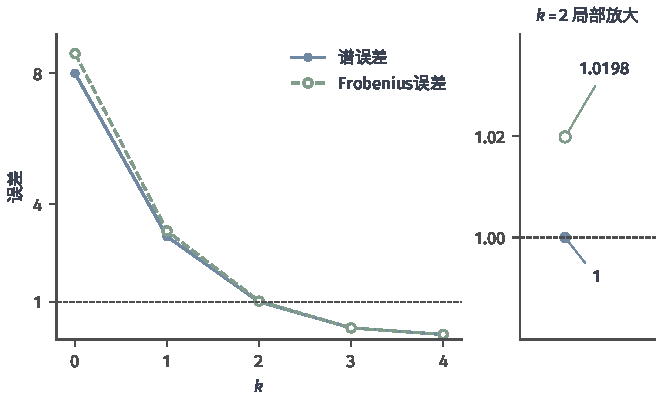
\includegraphics[width=112.0mm]{figures/01-mathematical-preliminaries-upper/02-linear-spaces/matplotlib/ch06-error-rank-curves/figure.pdf}
  \caption{固定奇异值$(8,3,1,0.2)$的最优误差曲线。给定横轴的秩可读出最低误差；
  给定水平误差阈值则寻找第一个满足要求的整数秩。$\tau=1$时，蓝色谱误差在
  $k=2$达标，绿色Frobenius误差要到$k=3$才达标。连线只辅助阅读，可行秩为整数。}
  \label{fig:ch06-error-rank-curves}
\end{figure}

\paragraph{中心化数据与PCA重构}

固定有限数据的重构是同一结论的实例。设$\bm X\in\mathbb R^{n\times d}$每行是一个样本，
先减去样本均值使每列之和为零。选择$\bm W^\top\bm W=\bm I_k$，低维坐标
$\bm Z=\bm X\bm W$，重构$\widehat{\bm X}=\bm Z\bm W^\top$，则
\begin{equation}
 \lVert\bm X-\bm X\bm W\bm W^\top\rVert_{\mathrm F}^2
 =\lVert\bm X\rVert_{\mathrm F}^2-\lVert\bm X\bm W\rVert_{\mathrm F}^2
 =\lVert\bm X\rVert_{\mathrm F}^2
 -\operatorname{tr}(\bm W^\top\bm X^\top\bm X\bm W).
 \label{eq:ls-pca-reconstruction}
\end{equation}
~\ref{sec:ls-quadratic-optimization}节的迹极值说明，最大化保留能量即取前$k$个右奇异
向量，重构恰为$\bm X_k$。这就是\term{主成分分析}（principal component analysis，PCA）
的有限矩阵形式；$n\geq2$时样本协方差$\bm X^\top\bm X/(n-1)$使保留方差总和为
$\lVert\bm X\bm W\rVert_{\mathrm F}^2/(n-1)$，最大化保留样本方差与最小化平方重构误差
等价。

例如四个中心化样本$(2,0)$、$(-2,0)$、$(0,1)$、$(0,-1)$，Gram矩阵为
$\operatorname{diag}(8,2)$。取$k=1$得$\bm W=(1,0)^\top$，坐标为$(2,-2,0,0)^\top$，
后两个样本都重构成零，误差平方为$2$。未中心化时，最强方向可能反映数据整体离原点的
位置而非围绕均值的变化；重构原始数据还应加回均值。把米改成毫米也会改变欧氏目标，是否
标准化必须由任务决定。最大样本方差不自动等于最有预测价值的方向，对总体协方差的估计
保证需要后续统计假设。

\paragraph{因子存储与作用代价}

以紧致因子存储$\bm A_k=\bm U_k\Sigma_k\bm V_k^\top$需要约$(m+n)k+k$个数，作用于一个
输入可先算$\bm V_k^\top\bm x$、按$\sigma_i$缩放、再乘$\bm U_k$。只有$k$相对两端
维数足够小时才真正节省存储和计算；小矩阵中因子开销可能更大。求SVD本身也有成本，不能
只统计后续乘法。噪声尺度若高于最后保留的奇异值，把$k$算得很精确也不等于方向可辨认，
方向可靠性由后续扰动分析章的谱隙条件判断。

\subsubsection{基于子空间压缩的近似求解}
\label{sec:ls-subspace-compression}

\paragraph{近似列空间与正交基}

完整SVD对超大矩阵代价过高。另一条路线把大矩阵近似拆成两步：先找一个$p$维近似列空间
$\operatorname{range}\bm Q$，$\bm Q\in\mathbb R^{m\times p}$满足
$\bm Q^\top\bm Q=\bm I_p$，$p\geq k$；再在这个小空间内解小规模问题。

\paragraph{压缩矩阵和小规模分解}

把$\bm A$投影到$\bm Q$上得到压缩矩阵$\bm C=\bm Q^\top\bm A\in\mathbb R^{p\times n}$，
对$\bm C$做薄SVD并截断到$k$项，$\bm C_k=\widehat{\bm U}_k\Sigma_k\widehat{\bm V}_k^\top$，
返回$\bm B=\bm Q\widehat{\bm U}_k\Sigma_k\widehat{\bm V}_k^\top$。大规模时只需要
$\bm Q$的乘法作用，不必显式形成完整$\bm U$。

\paragraph{子空间误差与截断误差的分离}

总误差由两部分独立组成：列空间未覆盖的残差$\lVert\bm A-\bm Q\bm Q^\top\bm A\rVert_2$，
加上压缩矩阵自身的截断尾能量。前者衡量找的子空间够不够大，后者衡量在子空间内保留几项，
两条预算分别分配，不能混为一谈。

\paragraph{随机化SVD的采样和计算流程}

\term{随机化SVD}（randomized SVD）只作为构造$\bm Q$的计算手段，本节给确定性流程，不给概率结论。取一个
$n\times p$的测试矩阵$\Omega$（元素独立抽样），计算$\bm Y=\bm A\Omega$，对$\bm Y$
作QR分解$\bm Y=\bm Q\bm R$得到正交基；随后压缩、小规模SVD、按上段返回候选。抽样把
寻找列空间的问题换成随机投影，成功概率与集中界由概率卷承担。

\paragraph{过采样、子空间迭代与访问次数}

$p=k+\ell$中$\ell$为过采样数，给弱方向留出余量。子空间迭代把$\bm Q$用
$(\bm A\bm A^\top)^q$刷新$q$次，每次需要正向与反向各访问$\bm A$一次，以访问次数
换取子空间精度；$q=0$就是单遍采样。过采样与迭代次数的选择依据概率卷的误差估计，
本节只记录流程与每步所需的矩阵作用。

\paragraph{Nyström的抽列与半正定重构}

半正定输入$\bm A\succeq0$另有\term{Nyström方法}（Nyström method）的抽列路径：按指标集$I$取出列块$\bm C=\bm A_{:,I}$与
交叉块$\bm W=\bm A_{I,I}$，用$\bm A\approx\bm C\bm W^{-1}\bm C^\top$重构，再对
$\bm C$作薄QR/SVD得到秩$k$候选。重构自动保持半正定；$\bm W$奇异时用伪逆或加小
扰动，属于数值实现细节。

\paragraph{确定性残差核验}

无论子空间如何得到，返回前都直接计算原矩阵残差
$\lVert\bm A-\bm B\rVert_{\mathrm F}$与子空间残差
$\lVert\bm A-\bm Q\bm Q^\top\bm A\rVert_2$，与既定预算比较；抽样随机性不改变核验
量，核验仍用原矩阵的确定性数值。

\paragraph{概率保证的后续入口}

期望误差、失败概率与集中不等式需要概率工具，可参考
\BookChapterRef{chap:probability-theory}{卷2《数学准备：概率、因果与决策》的概率基础章}；
本节只提供计算流程和确定性残差核验，不宣称随机子空间一定达到某条误差界。

\subsection{核范数惩罚的求解}
\label{sec:ls-nuclear-penalty-solve}

\paragraph{固定奇异值下的方向对齐}

回到~\eqref{eq:ls-nuclear-penalty-problem}。令$\bm B$的奇异值为$s_i\geq0$，展开
平方范数后方向只出现在交叉项$-\operatorname{tr}(\bm B^\top\bm A)$中。由
~\eqref{eq:ls-rearrangement-trace-bound}，固定$s_i$时令$\bm B$与$\bm A$的左右奇异
方向一致，交叉项最大、目标最小，方向子问题被方向对齐完全解决。

\paragraph{标量收缩与奇异值软阈值}

方向对齐后只剩逐个奇异值的独立问题
\begin{equation}
 \min_{s_i\geq0}\ \tfrac12(s_i-\sigma_i)^2+\lambda s_i.
 \label{eq:ls-soft-threshold-scalar}
\end{equation}
无约束极小点为$s_i=\sigma_i-\lambda$；若它小于零，非负约束把最优值压到$s_i=0$，故
\begin{equation}
 s_i=(\sigma_i-\lambda)_+=\max(\sigma_i-\lambda,0).
 \label{eq:ls-singular-value-soft-threshold}
\end{equation}
这是\term{奇异值软阈值}（singular value soft-thresholding）：保留方向上的奇异尺度被
$\lambda$整体压小，而不是像截断那样原值保留或整体舍弃。惩罚参数控制收缩幅度，产生的
实际秩取决于原谱，不等于直接指定$k$。

\paragraph{平衡因子表达与非凸求解边界}

核范数与因子平方惩罚之间有精确联系。
\begin{lemma}[核范数的因子分解表达]
\label{lem:matrix-analysis-nuclear-factorization}
设$\bm A\in\mathbb R^{m\times n}$，$r=\operatorname{rank}\bm A$。对任意正整数
$q\geq r$，
\begin{equation}
 \lVert\bm A\rVert_*
 =\min_{\substack{\bm L\in\mathbb R^{m\times q},\,
                  \bm R\in\mathbb R^{n\times q}\\
                  \bm L\bm R^\top=\bm A}}
   \tfrac12\bigl(\lVert\bm L\rVert_{\mathrm F}^2+\lVert\bm R\rVert_{\mathrm F}^2\bigr).
 \label{eq:matrix-analysis-nuclear-factorization}
\end{equation}
\end{lemma}
\begin{proof}
非零$\bm A$写紧致SVD$\bm P\Sigma\bm Q^\top$，取
$\bm L=\bm P\Sigma^{1/2}$、$\bm R=\bm Q\Sigma^{1/2}$，$q>r$补零列，两侧平方范数均为
$\sum_i\sigma_i$，故右侧不超过核范数。反过来令$\bm C=\bm P\bm Q^\top$，
$\lVert\bm C\rVert_2=1$，任意可行因子满足
$\lVert\bm A\rVert_*=\operatorname{tr}(\bm C^\top\bm A)
=\langle\bm C^\top\bm L,\bm R\rangle_{\mathrm F}
\leq\lVert\bm L\rVert_{\mathrm F}\lVert\bm R\rVert_{\mathrm F}
\leq\tfrac12(\lVert\bm L\rVert_{\mathrm F}^2+\lVert\bm R\rVert_{\mathrm F}^2)$，
依次使用Frobenius的Cauchy--Schwarz、混合次乘性与$2ab\leq a^2+b^2$。零矩阵取零因子。
\end{proof}
例如$\operatorname{diag}(4,1)$的平衡因子均为$\operatorname{diag}(2,1)$，每侧平方
能量$5$，平均后仍为核范数$5$；一侧乘$c$、另一侧除以$c$不改变乘积却一般增加总因子
能量，这就是“平衡”的含义。注意因子目标关于两侧联合变量仍非凸，恒等式不保证任意因子
算法达到全局最优；$q<r$时精确乘积约束不可行。
\section{张量低秩逼近}
\label{sec:ls-tensor-low-rank}

矩阵只有两个轴，SVD把它拆成两两配对的秩一项之和，并给出固定秩的全局最优。三个及以上
轴的\term{张量}（tensor，见~\ref{sec:ls-tensor-products}）有多种互不相同的“秩”概念，
矩阵截断SVD的最优性不能直接外推。本节先定义CP、Tucker与张量列车三种表示预算及其拟合
目标，再分别判断固定预算下最佳逼近是否存在，最后按模型给出只承担局部误差预算的求解
方法；全局非凸优化的一般理论留待后续最优化章。

\subsection{表示预算与目标}
\label{sec:ls-tensor-budget}

\subsubsection{CP表示}
\label{sec:ls-cp-representation}

\paragraph{多路分离的秩一张量}

一次读取同时依赖三组向量$\bm x\in\mathbb R^m$、$\bm y\in\mathbb R^n$、
$\bm z\in\mathbb R^p$时，完整参数数组需要$mnp$个数。取非零向量
$\bm a\in\mathbb R^m$、$\bm b\in\mathbb R^n$、$\bm c\in\mathbb R^p$，定义
\term{秩一张量}（rank-one tensor）
$(\bm a\otimes\bm b\otimes\bm c)_{i,j,k}=a_i b_j c_k$。有限求和可以分离：秩一读取等于
三个内积投影之积$(\bm a^\top\bm x)(\bm b^\top\bm y)(\bm c^\top\bm z)$，这一多路收缩
~\eqref{eq:linear-algebra-rank-one-contraction}已在5.11建立，
不必先生成$mnp$个乘积再读取，只需分别投影三组输入再乘三个标量。

\paragraph{秩一项之和与CP表示}

更丰富的参数写成若干可分离项之和，~\ref{sec:ls-tensor-products}节已引入
\term{CP表示}（CANDECOMP/PARAFAC representation）
\scite{math-kolda2009tensor}
\begin{equation}
 \mathcal W=\sum_{s=1}^r\bm a_s\otimes\bm b_s\otimes\bm c_s.
 \label{eq:ls-cp-sum}
\end{equation}
允许任意阶时按每条轴分别相乘；三阶是原型，更高阶逐条轴重复同一规则。

\paragraph{CP秩与因子规模}

能表示数组的最少非零秩一项数称为该标量域上的\term{张量秩}（tensor rank，CP秩），
零数组的秩取零。给出$r$项只说明秩至多为$r$，项之间可能相消；它与数组的轴数完全不同。
存储量从$mnp$变为$r(m+n+p)$，只有后者较小时才节省；小尺寸数组上因子参数反而更多。

\paragraph{因子缩放和排列的不唯一}

每一项内部可以把$\bm a_s$乘$c$、$\bm c_s$除以$c$而乘积不变，项的次序也可以任意
排列；与SVD不同，CP因子之间没有正交约束，同一数组的因子组不唯一，也不存在标准的
“左右奇异向量”。

\paragraph{CP预算下的拟合目标}

固定项数$r$，在所有CP秩不超过$r$的张量中最小化Frobenius距离：
\begin{equation}
 \min_{\{\bm a_s,\bm b_s,\bm c_s\}_{s=1}^r}
 \lVert\mathcal T-\sum_{s=1}^r\bm a_s\otimes\bm b_s\otimes\bm c_s\rVert_{\mathrm F}^2.
 \label{eq:ls-cp-fitting-objective}
\end{equation}
目标关于全体因子联合非凸，下面的交替方法只保证每步局部改进，不宣称全局最佳。

\subsubsection{Tucker表示}
\label{sec:ls-tucker-representation}

\paragraph{按轴展开与列空间}

Tucker模型不要求逐项分离，而是给每条轴各找一个子空间。把张量沿第$n$轴展开成矩阵
$\mathcal T_{(n)}\in\mathbb R^{I_n\times(\prod_{j\neq n}I_j)}$，其列空间就是第$n$
轴使用的方向集合。

\paragraph{各轴子空间与多线性秩}

第$n$个展开矩阵的秩$r_n=\operatorname{rank}\mathcal T_{(n)}$称为该轴的
\term{单秩}，元组$(r_1,\ldots,r_N)$为\term{多线性秩}（multilinear rank）。
它是各轴独立计数的，不需要各项跨轴配对。

\paragraph{基变换后的核心张量}

取各轴列空间的标准正交基$\bm U_n\in\mathbb R^{I_n\times r_n}$，经$n$模积把坐标
变换到基上，剩余的轴间耦合由\term{核心张量}（core tensor）
$\mathcal G\in\mathbb R^{r_1\times\cdots\times r_N}$记录，整体结构称
\term{Tucker表示}（Tucker decomposition）：
\begin{equation}
 \mathcal T\approx\mathcal G\times_1\bm U_1\times_2\cdots\times_N\bm U_N.
 \label{eq:ls-tucker-form}
\end{equation}

\paragraph{Tucker表示与参数规模}

参数规模为$\sum_n I_n r_n+\prod_n r_n$：各轴基向量加上核心。当$r_n\ll I_n$时比
稠密数组$\prod_n I_n$小得多，核心本身仍是小稠密数组。

\paragraph{多线性秩预算下的误差目标}

固定各轴上界$(k_1,\ldots,k_N)$，在$\operatorname{rank}\mathcal T_{(n)}\leq k_n$
的张量中最小化Frobenius距离。约束是各轴展开矩阵的秩条件，与CP的逐项分离条件不同。

\subsubsection{张量列车表示}
\label{sec:ls-tt-representation}

\paragraph{前后轴切分与矩阵展开}

\term{张量列车}（tensor train，TT）沿固定轴次序逐次切分：把前$j$条轴与其余轴分开，
把张量展开为矩阵$\mathcal T_{[1:j]}\in\mathbb R^{(\prod_{i\leq j}I_i)\times
(\prod_{i>j}I_i)}$，其秩记录这一切分需要多少连接指标。

\paragraph{逐次分解与中间连接指标}

$N$阶数组写成一串$N$个\term{TT核心}（TT core）
$\mathcal G^{(j)}\in\mathbb R^{r_{j-1}\times I_j\times r_j}$，相邻核心通过中间连接
指标$r_j$衔接，$r_0=r_N=1$。

\paragraph{TT核心与张量恢复}

逐元素恢复为
\begin{equation}
 t_{i_1\cdots i_N}
 =\sum_{a_1,\ldots,a_{N-1}}
 \mathcal G^{(1)}_{i_1,a_1}
 \mathcal G^{(2)}_{a_1,i_2,a_2}\cdots
 \mathcal G^{(N)}_{a_{N-1},i_N}.
 \label{eq:ls-tt-recovery}
\end{equation}

\paragraph{TT秩和轴次序}

$r_j$是第$j$个切分展开矩阵的秩，称为\term{TT秩}（TT rank）。它依赖轴次序：交换两条
轴可能改变所有$r_j$，选次序本身是一个预处理问题。

\paragraph{存储规模与拟合目标}

存储量为$\sum_j I_j r_{j-1}r_j$，避开了核心的全张量乘积；固定TT秩上界后最小化
Frobenius残差，求解方法见~\ref{sec:ls-tt-truncation}。

\subsection{存在性与选解}
\label{sec:ls-tensor-existence}

\paragraph{固定CP秩约束下的不取到现象}

与矩阵不同，集合$\{\mathcal W:\operatorname{rank}_{\mathrm{CP}}\mathcal W\leq r\}$
一般不是闭集：一串CP秩不超过$r$的张量可以收敛到CP秩$r+1$的极限，极限不在集合内。
因此固定$r$的最佳CP逼近可能只达到下确界而不取到，即最小距离不存在最小点；实张量上
这一现象真实发生，不能用“取极限”悄悄补上。需要存在性保证时应改用下面两类闭约束。

\paragraph{固定多线性秩上界与闭性}

条件$\operatorname{rank}\mathcal T_{(n)}\leq k_n$对每个$n$都是展开矩阵的
$(k_n+1)$阶子式同时为零，有限个矩阵秩条件的交是闭集。取有界极小化序列，由
~\ref{thm:ls-extreme-value}在闭有界集上取极限，最佳Tucker候选存在。

\paragraph{固定TT秩上界与闭性}

TT秩上界同样是有限个切分展开矩阵的秩条件，集合闭，最佳TT逼近存在；闭性来自矩阵秩条件，
不依赖逐项分离。

\paragraph{因子非唯一与逼近对象的非唯一}

即使逼近张量存在，因子也可能不唯一：CP有缩放与排列自由度，Tucker各轴基可右乘正交矩阵，
TT核心有 gauge 变换。弱谱条件下最佳逼近张量本身也可能不唯一，存在性结论不附带
唯一性保证。

\subsection{求解方法}
\label{sec:ls-tensor-solve}

\subsubsection{CP因子拟合}
\label{sec:ls-cp-alternating}

\paragraph{固定其他因子后的线性作用}

交替最小二乘每次只更新一条轴的因子。固定$\{\bm b_s,\bm c_s\}$，目标对
$\bm a_s$们线性：把指标$(j,k)$逐行排列，系数矩阵的第$s$列为
$\bm b_s\otimes\bm c_s$（Khatri--Rao列），待求向量由$\bm a_s$堆叠而成。

\paragraph{单因子最小二乘的构造}

这一步化为一个普通线性最小二乘问题，可直接使用~\ref{sec:ls-least-squares}节的正规
方程、QR或SVD工具求解，只替换待求因子，其他因子保持不变。

\paragraph{因子更新与循环次序}

按轴轮流更新：先解所有$\bm a_s$，再固定它们解$\bm b_s$，再解$\bm c_s$，循环往复；
每次更新后对列归一化并把尺度吸收到下一条轴，消除缩放自由度带来的漂移。

\paragraph{每步目标变化与停止}

每次单因子最小二乘都使平方残差不增，目标序列单调下降；以相对残差变化小于阈值或达到
轮数为停止条件。单调下降只说明不退步，不说明到达全局最小。

\paragraph{因子增大和数值退化}

因子列之间接近共线时，单因子正规方程病态，解被放大；归一化、列正交检查与必要时的
正则化属于数值实现，不能消除模型本身的非凸性。

\paragraph{局部停止与全局最优的区别}

停点只满足“固定其他因子时本条轴最优”的驻点条件，是局部极小；不同初值可能停在不同
驻点。全局最佳CP逼近的存在性与求解属于完整非凸优化理论，留待后续最优化章，本节不宣称
交替法给出全局解。

\subsubsection{Tucker截断}
\label{sec:ls-hosvd}

\paragraph{各轴展开的SVD}

对每个展开矩阵$\mathcal T_{(n)}$做SVD，取前$k_n$个左奇异向量组成$\bm U_n$，
这一步复用~\ref{thm:ls-svd-existence}，不重新构造SVD。

\paragraph{主子空间选择与核心计算}

核心由投影得到$\mathcal G=\mathcal T\times_1\bm U_1^\top\cdots\times_N\bm U_N^\top$，
各轴独立选取主子空间。

\paragraph{截断张量的重构}

截断候选$\widetilde{\mathcal T}
=\mathcal G\times_1\bm U_1\cdots\times_N\bm U_N$，即\term{HOSVD}（higher-order SVD，高阶SVD）截断。

\paragraph{各轴误差与总误差界}

第$n$轴舍弃的展开能量为$\sum_{i>k_n}\sigma_i(\mathcal T_{(n)})^2$；总Frobenius
误差平方被各轴舍弃能量之和控制：
\begin{equation}
 \lVert\mathcal T-\widetilde{\mathcal T}\rVert_{\mathrm F}^2
 \leq\sum_{n=1}^N\sum_{i>k_n}\sigma_i(\mathcal T_{(n)})^2.
 \label{eq:ls-hosvd-error-bound}
\end{equation}
这是各轴独立截断的累计预算，不是联合最优误差。

\paragraph{秩预算与存储代价}

按各轴尾能量分别选定$k_n$，再核对参数规模$\sum_n I_n k_n+\prod_n k_n$是否落在
预算内；核心随$\prod_n k_n$增长，维数较多时核心本身可能成为瓶颈。

\paragraph{HOSVD的非最优边界}

各轴子空间独立选取，没有联合最小化总残差，因此HOSVD截断不保证达到固定多线性秩下的
全局最佳；迭代修正各轴基可以改善残差，但仍是局部改进，不改变非最优边界。

\subsubsection{张量列车截断}
\label{sec:ls-tt-truncation}

\paragraph{轴顺序与首次展开}

先固定轴次序，把第$1$轴与其余轴分开展开为矩阵，做SVD并按$r_1$截断。

\paragraph{截断SVD与首个TT核心}

薄SVD给出左因子与缩放，前者整理为首个TT核心$\mathcal G^{(1)}$，右因子矩阵传给下一步。

\paragraph{余因子传递与逐次展开}

把余因子矩阵沿第$2$轴再次切分、SVD、截断，得到$\mathcal G^{(2)}$并继续传递；逐次
进行到最后一条轴，每个切分复用矩阵截断SVD的尾能量结论。

\paragraph{局部误差的累计控制}

每一步截断都引入一个尾能量，总误差平方不超过各步尾能量之和，误差沿链条累计而非抵消。

\paragraph{总误差预算的逐步分配}

把总预算$\tau^2$分配到各步$\tau_j^2$，$\sum_j\tau_j^2\leq\tau^2$，每步只在
自身预算内截断；预算分配影响各$r_j$的大小。

\paragraph{TT秩与中间存储}

记录每步$r_j$与中间矩阵尺寸，避免连接指标无节制增长；中间存储随
$\prod_{i\leq j}I_i$与$r_j$变化，是TT实现的主要开销。

\paragraph{重构残差与非最优边界}

由核心按~\eqref{eq:ls-tt-recovery}重构后直接计算残差$\lVert\mathcal X-\widehat{\mathcal X}\rVert_{\mathrm F}$，
并与各次局部尾能量之和比较；逐次贪心截断不联合最优，局部误差累计得到的是预算保证而非最佳值，
残差超出预算时应回退上一层连接秩而不是继续贪心。

\subsection{结果核验}
\label{sec:ls-tensor-verification}

\paragraph{重构残差与表示规模}

返回候选前分别计算Frobenius重构残差$\lVert\mathcal X-\widehat{\mathcal X}\rVert_{\mathrm F}$
与实际参数量，与原定预算逐项比较。三套口径的计数不同，不能共用一个总数：CP为
$R\sum_{i=1}^d n_i$；Tucker为$\sum_{i=1}^d n_i r_i+\prod_{i=1}^d r_i$；TT为
$\sum_{i=1}^d n_i r_{i-1}r_i$（约定$r_0=r_d=1$）。预算通常同时给定残差上界$\varepsilon$
与参数量上界$N$，两项都满足才算交差；例如$n_i=100$、$d=4$、$R=10$时CP需$4000$个数，
而同维满张量为$10^8$，压缩比由计数直接算出，不能只凭"低秩"宣称节省。

\paragraph{因子增大、数值退化与停止}

交替法每轮记录残差序列$\rho_t=\lVert\mathcal X-\widehat{\mathcal X}^{(t)}\rVert_{\mathrm F}$
与轮数$t$；同时检查因子列范数是否失控（归一化后单列能量占比畸高）、相邻因子是否近似共线
（$\bm a_r^{(i)\top}\bm a_{r+1}^{(i)}/(\lVert\bm a_r^{(i)}\rVert\lVert\bm a_{r+1}^{(i)}\rVert)$
接近$1$）。当$\rho_t-\rho_{t-1}<\delta\,\rho_{t-1}$或达到轮数上限即停，停点只作为局部结果
报告，不写成全局最佳；退化发生时应重新初始化或降低$R$，而不是把局部残差当最优误差。
\section{正交映射逼近}
\label{sec:ls-orthogonal-approximation}

第~\ref{sec:ls-matrix-low-rank}节限制候选的秩，本节限制候选的几何性质：要求它保持长度。
有噪声的坐标变换可能不再是旋转，任务是在所有保持长度的矩阵中找一个离它最近的，包括
方阵正交、矩形部分等距与定向（行列式为正）三种约束。方向配对不等式在本节直接复用，
不重新证明。

\subsection{目标与约束}
\label{sec:ls-orthogonal-objective}

\paragraph{最近正交矩阵与对应点对齐}

给定$\bm A\in\mathbb R^{d\times d}$，在正交矩阵中最小化Frobenius距离
\begin{equation}
 \min_{\bm R^\top\bm R=\bm I_d}\ \lVert\bm A-\bm R\rVert_{\mathrm F}^2.
 \label{eq:ls-nearest-orthogonal-objective}
\end{equation}
形状对齐中更常见的是两组已对应列向量$\bm X,\bm Y\in\mathbb R^{d\times n}$，求
$\bm R$使$\lVert\bm R\bm X-\bm Y\rVert_{\mathrm F}^2$最小，即\term{正交Procrustes问题}
（orthogonal Procrustes problem）。

\paragraph{列正交、正交与定向约束}

$\bm Q\in\mathbb R^{m\times n}$（$m\geq n$）只要求$\bm Q^\top\bm Q=\bm I_n$，
称为列正交或\term{部分等距}（partial isometry），它在$\mathbb R^n$上保持长度但
$\mathbb R^m$维数有余量；方阵$\bm R^\top\bm R=\bm I$同时给出$\bm R\bm R^\top=\bm I$。
定向约束再加$\det\bm R=1$，候选限于特殊正交群$\mathrm{SO}(d)$，排除反射。

\paragraph{输入误差尺度与目标矩阵}

默认用Frobenius距离，它把每条输出方向的偏差平方累计；谱范数口径下最优解可能不唯一，
见~\ref{sec:ls-orthogonal-existence}。$\bm A$可以奇异，奇异方向留有的自由度正是
非唯一性的来源。

\subsection{存在性与唯一性}
\label{sec:ls-orthogonal-existence}

\paragraph{维数条件与可行性}

列正交要求$m\geq n$；$m<n$时不存在$\bm Q^\top\bm Q=\bm I_n$，问题不可行，应改求
$\bm Q\bm Q^\top=\bm I_m$的行正交版本。方阵正交与$\mathrm{SO}(d)$对任意$d$非空。

\paragraph{有限维闭有界约束与极值存在}

正交集合由$\bm R^\top\bm R=\bm I$定义，是有限维中的闭有界集（各列单位长度且互相
正交），Frobenius距离连续，由~\ref{thm:ls-extreme-value}最小点存在；$\mathrm{SO}(d)$
是其闭子集，同样存在最小点。

\paragraph{秩亏、奇异值与非唯一性}

$\bm A$有零奇异值或重复弱奇异值时，规范部分等距因子在零方向上不受原矩阵约束，最优
矩阵可能不唯一。例如$\operatorname{diag}(2,0)$的规范因子$\bm Q=\operatorname{diag}(1,0)$，
而正交延拓$\operatorname{diag}(1,1)$与$\operatorname{diag}(1,-1)$乘以同一半正定
因子都给原矩阵；延拓自由不等于规范因子本身不唯一。

\subsection{求解方法}
\label{sec:ls-orthogonal-solve}

\subsubsection{基于SVD的直接求解}
\label{sec:ls-orthogonal-svd}

\paragraph{距离目标的迹配对展开}

展开平方距离：
\begin{equation}
 \lVert\bm A-\bm R\rVert_{\mathrm F}^2
 =\lVert\bm A\rVert_{\mathrm F}^2+d-2\operatorname{tr}(\bm R^\top\bm A),
 \label{eq:ls-orthogonal-trace-expand}
\end{equation}
前两项与$\bm R$无关，故最小误差等价于最大化$\operatorname{tr}(\bm R^\top\bm A)$。

\paragraph{SVD方向对齐与极因子}

设$\bm A=\bm U\Sigma\bm V^\top$，令$\bm W=\bm U^\top\bm R\bm V$，则$\bm W$正交，
$\operatorname{tr}(\bm R^\top\bm A)=\operatorname{tr}(\bm W\Sigma)$。由
~\eqref{eq:ls-rearrangement-trace-bound}，配对上界为$\sum_i\sigma_i$，在
$\bm W=\bm I$即$\bm R=\bm U\bm V^\top$时取等。这一因子就是\term{极分解}
（polar decomposition）\label{def:matrix-analysis-polar-decomposition}
$\bm A=\bm Q\bm H$的规范部分：
\begin{equation}
 \bm A=\bm Q\bm H,\qquad
 \bm H=(\bm A^\top\bm A)^{1/2}=\bm V\Sigma\bm V^\top\succeq0,\qquad
 \bm Q=\bm U\bm V^\top.
 \label{eq:matrix-analysis-polar-decomposition}
\end{equation}
$\bm H$由唯一半正定平方根确定，$\bm Q$在$\operatorname{range}\bm H$上被
$\bm A=\bm Q\bm H$确定，在其正交补取零，故规范$\bm Q$唯一。

\paragraph{矩形部分等距与正交延拓}

$m>n$或秩亏时，规范$\bm Q=\bm U_r\bm V_r^\top$只在$(\ker\bm A)^\perp$上保持长度，
并在$\ker\bm A$上取零；把它延拓为整个空间的正交矩阵需要任选零方向的标准正交基，
延拓不唯一。迭代趋于规范部分等距，并不自动给出任意正交延拓。

\paragraph{对应点对齐的Procrustes化简}

对齐$\lVert\bm R\bm X-\bm Y\rVert_{\mathrm F}^2$展开为
$\lVert\bm Y\rVert_{\mathrm F}^2+\lVert\bm X\rVert_{\mathrm F}^2
-2\operatorname{tr}(\bm R^\top\bm Y\bm X^\top)$，对$\bm M=\bm Y\bm X^\top$
作SVD$\bm M=\widehat{\bm U}\widehat\Sigma\widehat{\bm V}^\top$，同一配对论证给
$\bm R_*=\widehat{\bm U}\widehat{\bm V}^\top$。若还允许平移，先减去各组均值
$\bar{\bm x},\bar{\bm y}$，求得$\bm R_*$后取
$\bm t_*=\bar{\bm y}-\bm R_*\bar{\bm x}$。

\paragraph{定向约束下的符号修正}

限制$\det\bm R=1$时，令$s=\det(\bm U\bm V^\top)\in\{-1,1\}$。$s=1$直接取
$\bm R=\bm U\bm V^\top$；$s=-1$时实正交矩阵至少有一个特征值$-1$，其余特征值实部
不超过$1$，故$\operatorname{tr}\bm W\leq d-2$，把最小奇异值方向的符号翻转即可达到
\label{sec:linear-algebra-orthogonal-procrustes}：
\begin{equation}
 \bm R_*=\bm U\operatorname{diag}(1,\ldots,1,s)\bm V^\top
 \in\argmin_{\bm R\in\mathrm{SO}(d)}\lVert\bm A-\bm R\rVert_{\mathrm F}.
 \label{eq:linear-algebra-nearest-rotation}
\end{equation}
行列式修正应放在最小奇异值方向，而不是任意改一列。例如$\bm A=\operatorname{diag}(2,1,-1/2)$
的最近正交矩阵为$\operatorname{diag}(1,1,-1)$，但它是反射；限制为旋转后上式给
$\bm R_*=\bm I$，平方误差$1+(3/2)^2=13/4$。定向限制确实增加误差，不能称作无代价
的修正\scite{math-lawrence2019kabsch}。

\paragraph{最优性与非唯一边界}

严格奇异值间隙使规范因子唯一；零奇异值或等奇异值留下自由度，最优矩阵不唯一。谱范数口径
下即使有间隙也可能多个最优，与~\ref{sec:ls-low-rank-existence}的结论一致。

\subsubsection{基于乘法迭代的近似求解}
\label{sec:ls-polar-iteration}

\paragraph{极因子的乘法近似需求}

完整SVD代价较高；只需要极因子时，可以构造只用矩阵乘法的多项式更新，避免显式分解。

\paragraph{Newton--Schulz多项式更新}

对标量缩放到$\lVert\bm A\rVert_2\leq1$附近的$\bm X_0=\bm A/\beta$，固定更新
\begin{equation}
 \bm X_{t+1}=\tfrac12\bm X_t(3\bm I-\bm X_t^\top\bm X_t).
 \label{eq:ls-newton-schulz-polar}
\end{equation}
它的不动点满足$\bm X^\top\bm X=\bm I$（矩形时为部分等距），与逆迭代的多项式校正
同一类构造，收敛域与二次递推证明在~\ref{sec:ls-matrix-function-iteration-convergence}
节完成。

\paragraph{奇异方向保持与尺度变化}

更新与$\bm A$共用右奇异方向，对每个奇异值$s$化为标量递推
$s_{t+1}=\tfrac12s_t(3-s_t^2)$；$0<s<\sqrt3$时它把$s$推向$1$，零方向保持零，
方向不发生混合。

\paragraph{输入缩放与初始区间}

取$\beta\geq\lVert\bm A\rVert_2$（例如$\beta=\lVert\bm A\rVert_{\mathrm F}$）把谱
压到可检查区间，初始化无需分解；超出区间会使标量映射发散，不能省略缩放。

\paragraph{零方向与部分等距输出}

零奇异方向在迭代中保持零，极限是规范部分等距；迭代不供应任意正交延拓，需要延拓时另行
补基。

\paragraph{有限步整形与极限求解的区别}

有限次迭代只得到近似极因子，不是精确解；每步三次矩阵乘法，停止量为正交残差
$\lVert\bm X_t^\top\bm X_t-\bm I\rVert$，与极限方程$\bm X^\top\bm X=\bm I$分开评价。
标量递推在$s_t$接近$1$时二次收敛，残差平方量级下降，故达到给定容限所需步数与初始
距离有关，不能用固定步数代替收敛判断。

\subsection{结果核验}
\label{sec:ls-orthogonal-verification}

\paragraph{正交残差与部分等距残差}

方阵核验$\lVert\bm R^\top\bm R-\bm I\rVert$；矩形候选核验
$\lVert\bm Q^\top\bm Q-\bm I_n\rVert$与$\bm Q\bm Q^\top$是否等于目标投影。
定向约束再检查$\det\bm R=1$。

\paragraph{作用误差、目标差与计算代价}

同时计算目标差$\lVert\bm A-\bm R\rVert_{\mathrm F}^2=\sum_i(\sigma_i-1)^2$并与该理论
最小值比较，两者之差即方向未对齐的代价。点对问题再把$\lVert\bm A\bm R-\bm B\rVert_{\mathrm F}$
与$\lVert\bm B\rVert_{\mathrm F}$归一，得到可解释的对齐比例。乘法迭代记录每步矩阵乘法次数，
与完整SVD的$O(mn\min(m,n))$建立代价按规模比较；迭代收敛到什么精度也由残差
$\lVert\bm X^\top\bm X-\bm I\rVert$的截断水平决定，不写成精确等于极因子。
\section{对称与谱约束逼近}
\label{sec:ls-symmetric-spectral-approximation}

~\ref{sec:ls-orthogonal-approximation}节的正交集合不是凸集，最优解可能不唯一；本节处理
三类凸约束：最近对称矩阵、最近半正定矩阵与谱范数球内的最近矩阵。凸集合上的平方距离
有唯一最小点，求解归结为对称化、特征值截断与奇异值裁剪。

\subsection{目标与约束}
\label{sec:ls-symmetric-objective}

\paragraph{最近对称矩阵与最近半正定矩阵}

给定$\bm A\in\mathbb R^{d\times d}$，第一类在对称矩阵集合
$\operatorname{Sym}_d=\{\bm S:\bm S=\bm S^\top\}$中找最近点；第二类\term{最近半正定矩阵}
（nearest positive semidefinite matrix）在半正定锥
$\mathbb S_+^d=\{\bm P:\bm P=\bm P^\top,\ \bm x^\top\bm P\bm x\geq0\ \forall\bm x\}$
中找最近点，误差均取Frobenius平方距离。

\paragraph{谱范数球与Frobenius距离}

第三类约束把候选限制在\term{谱范数球}（spectral norm ball）$\{\bm B:\lVert\bm B\rVert_2\leq\rho\}$内，
$\rho>0$，同样最小化$\lVert\bm A-\bm B\rVert_{\mathrm F}^2$。它限制的是最大奇异值，
与对称约束限制特征值符号是两类问题。

\subsection{存在性与唯一性}
\label{sec:ls-symmetric-existence}

\paragraph{闭凸约束与平方距离的唯一最小点}

对称集合是线性子空间，半正定锥与谱范数球是凸集：两对称矩阵的线段仍对称；两个半正定
矩阵的凸组合$(1-t)\bm P+t\bm Q$仍半正定；谱范数是范数，单位球凸。平方距离
$\lVert\bm A-\bm B\rVert_{\mathrm F}^2$是严格凸函数，凸集上的最小点唯一。可行集闭，
极小化序列有界（谱球直接有界；半正定锥上最近点满足$\lVert\bm P\rVert_{\mathrm F}
\leq\lVert\bm A\rVert_{\mathrm F}$，故序列有界），由~\ref{thm:ls-extreme-value}
取到极值。

\paragraph{特征值约束与奇异值约束的区别}

对称与半正定问题在实对称谱坐标中求解，使用~\ref{thm:ls-real-symmetric-spectral}的
特征值；谱范数球问题使用奇异值。前者方向被限制在输入自己的特征向量上，后者允许两端
方向分别配对，不能把特征值截断直接套到非对称输入。

\subsection{求解方法}
\label{sec:ls-symmetric-solve}

\subsubsection{对称与半正定约束}
\label{sec:ls-psd-projection}

\paragraph{对称部分与反对称部分}

任意$\bm A$唯一分解为对称部分与反对称部分：
\begin{equation}
 \bm A_{\mathrm s}=\tfrac12(\bm A+\bm A^\top),\qquad
 \bm A_{\mathrm k}=\tfrac12(\bm A-\bm A^\top),
 \qquad \bm A=\bm A_{\mathrm s}+\bm A_{\mathrm k}.
 \label{eq:ls-skew-split}
\end{equation}

\paragraph{Frobenius误差的正交分离}

反对称矩阵与对称矩阵在Frobenius配对下正交：
$\operatorname{tr}(\bm A_{\mathrm k}^\top\bm A_{\mathrm s})=0$，故对任意对称$\bm S$，
\begin{equation}
 \lVert\bm A-\bm S\rVert_{\mathrm F}^2
 =\lVert\bm A_{\mathrm k}\rVert_{\mathrm F}^2
 +\lVert\bm A_{\mathrm s}-\bm S\rVert_{\mathrm F}^2.
 \label{eq:ls-symmetric-orthogonal-separation}
\end{equation}
第一项与$\bm S$无关。

\paragraph{最近对称矩阵}

第二项在$\bm S=\bm A_{\mathrm s}$时为零，故最近对称矩阵就是对称部分
$\bm S_*=\tfrac12(\bm A+\bm A^\top)$，反对称分量$\bm A_{\mathrm k}$无法由对称候选
消除，全部计入误差。

\paragraph{半正定约束下的谱坐标}

对半正定问题，先取$\bm A_{\mathrm s}$的实对称谱分解
$\bm A_{\mathrm s}=\bm Q\Lambda\bm Q^\top$，$\Lambda=\operatorname{diag}(\lambda_i)$。
在谱坐标中对称候选$\bm S=\bm Q\operatorname{diag}(\mu_i)\bm Q^\top$，半正定要求
$\mu_i\geq0$，误差平方为$\sum_i(\lambda_i-\mu_i)^2$，各$\mu_i$独立。

\paragraph{特征值非负截断}

每个标量问题$\min_{\mu_i\geq0}(\lambda_i-\mu_i)^2$的解为$\mu_i=\max(\lambda_i,0)$，
故
\begin{equation}
 \bm P_*=\bm Q\operatorname{diag}(\lambda_1^+,\ldots,\lambda_d^+)\bm Q^\top,
 \qquad \lambda_i^+=\max(\lambda_i,0).
 \label{eq:ls-nearest-psd}
\end{equation}
负特征值截为零而不是取绝对值，因为半正定只要求非负，把负号翻正会改变方向配对并增大
距离。

\paragraph{可行性与最优性核验}

核验$\bm P_*\succeq0$（所有$\mu_i\geq0$）与残差$\lVert\bm A-\bm P_*\rVert_{\mathrm F}$；
例如$\bm A=\operatorname{diag}(2,-1)$的最近半正定矩阵为$\operatorname{diag}(2,0)$，
误差平方为$1$，而$\operatorname{diag}(2,1)$不是可行点且距离更大。

\subsubsection{谱范数约束}
\label{sec:ls-spectral-ball}

\paragraph{谱范数球与奇异值上界}

$\lVert\bm B\rVert_2\leq\rho$等价于$\bm B$的每个奇异值$s_i\leq\rho$，由
~\ref{thm:ls-svd-existence}的奇异值定义直接得到。

\paragraph{迹配对与最优方向}

展开$\lVert\bm A-\bm B\rVert_{\mathrm F}^2$，方向只出现在交叉项
$-\operatorname{tr}(\bm B^\top\bm A)$。由~\eqref{eq:ls-rearrangement-trace-bound}，
固定奇异值时让$\bm B$与$\bm A$使用相同左右奇异方向最优。

\paragraph{标量区间上的最近值}

方向对齐后，每个奇异值独立求解
$\min_{0\leq s_i\leq\rho}(s_i-\sigma_i)^2$，解为
$s_i=\min(\sigma_i,\rho)$：$\sigma_i<\rho$时保留原值，超过$\rho$的压到边界。

\paragraph{奇异值裁剪与矩阵恢复}

设$\bm A=\bm U\Sigma\bm V^\top$，返回
\begin{equation}
 \bm B_*=\bm U\operatorname{diag}(\min(\sigma_1,\rho),\ldots,
 \min(\sigma_q,\rho))\bm V^\top.
 \label{eq:ls-spectral-clipping}
\end{equation}

\paragraph{最优性与边界核验}

核验$\lVert\bm B_*\rVert_2\leq\rho$与残差$\lVert\bm A-\bm B_*\rVert_{\mathrm F}^2
=\sum_i(\sigma_i-\min(\sigma_i,\rho))^2$；落在边界上的方向$s_i=\rho$对应被裁剪的
大奇异值，内部方向$s_i=\sigma_i<\rho$保持原值，两者不要混淆。例如$\sigma=(3,1)$、
$\rho=2$时裁剪为$(2,1)$，残差平方为$(3-2)^2=1$，第二个奇异值未被改动。

\subsection{结果核验}
\label{sec:ls-symmetric-verification}

\paragraph{可行性残差与逼近误差}

分别核对约束条件：对称差$\lVert\bm S-\bm S^\top\rVert_{\mathrm F}$、半正定特征值下界
$\min_i\lambda_i(\bm P)\geq0$、谱范数上界$\lVert\bm B\rVert_2\leq\rho$，再报告Frobenius
逼近误差。三类误差分开列：可行性残差应在数值精度内为零，逼近误差才是与$\bm A$的距离；
可行性不满足时误差数字没有意义。例如把$\bm A=\operatorname{diag}(2,-1)$投影到半正定锥，
$\bm P_*=\operatorname{diag}(2,0)$，可行性残差为零而逼近误差平方恰为$(-1)^2=1$，
二者不可合并成一个数。

\paragraph{正交集合与凸谱约束的区别}

正交Stiefel集合非凸（~\ref{sec:ls-orthogonal-approximation}），可能多解；本节三类
集合凸，解唯一。一般凸投影理论、不等式约束优化与次梯度方法留待后续最优化章，这里只解
当前三个具体问题。
\section{矩阵方程}
\label{sec:ls-matrix-equations}
\label{sec:linear-algebra-matrix-equations}

前面各节的未知量是向量或约束矩阵，本节未知量本身是一张矩阵：左乘对未知矩阵的各行作线性
组合，右乘对各列作线性组合。先建立矩阵上的线性作用与相容、可逆条件，再用向量化与实Schur
块求解；本章只作代数判据、对称结构和正定结果核验，不使用长期衰减定理构造正定解。

\subsection{方程与线性算子}
\label{sec:ls-matrix-equation-types}

\paragraph{单侧、双侧与多项矩阵作用}

单侧方程$\bm A\bm X=\bm C$只从左边作用；$\bm X\bm B=\bm C$只从右边作用；双侧
$\bm A\bm X\bm B=\bm C$两端同时约束。多项作用的典型是\term{Sylvester方程}
（Sylvester equation）
\begin{equation}
 \bm A\bm Z+\bm Z\bm B=\bm C,
 \label{def:matrix-analysis-sylvester-equation}
\end{equation}
给定$\bm A\in\mathbb R^{m\times m}$、$\bm B\in\mathbb R^{n\times n}$、
$\bm C\in\mathbb R^{m\times n}$，求$\bm Z\in\mathbb R^{m\times n}$。固定作用矩阵后，
这些方程关于未知矩阵都是线性的。

\paragraph{向量化与Kronecker表示}

~\ref{sec:ls-kronecker-products}节的向量化恒等式
$\operatorname{vec}(\bm A\bm X\bm B)
=(\bm B^\top\otimes\bm A)\operatorname{vec}\bm X$把矩阵方程编码为普通向量方程；
Sylvester方程向量化为
\begin{equation}
 (\bm I_n\otimes\bm A+\bm B^\top\otimes\bm I_m)\operatorname{vec}\bm Z
 =\operatorname{vec}\bm C.
 \label{eq:ls-sylvester-vectorized}
\end{equation}
向量系统的求解方法可以直接复用，但大规模时应利用左右乘法，避免存储$mn\times mn$的
Kronecker矩阵。

\paragraph{Sylvester与Lyapunov方程}

\term{Lyapunov方程}是Sylvester的对称特化：连续型
$\bm A\bm P+\bm P\bm A^\top=\bm W$，离散型
$\bm A^\top\bm P\bm A-\bm P=\bm Q$，右端$\bm W,\bm Q$对称半正定，未知量要求对称。
它的代数可逆性与对称性在本节判断；由系统衰减构造正定解的构造不属于本章。

\subsection{存在性与唯一性}
\label{sec:ls-matrix-equation-existence}

\paragraph{单侧与双侧方程的相容性}

$\bm A\bm X=\bm C$相容当且仅当$\bm C$的每一列都在$\operatorname{range}\bm A$内，
即$\operatorname{rank}[\bm A\ \bm C]=\operatorname{rank}\bm A$。$\bm A\bm X\bm B=\bm C$
相容要求$\bm C$落在$\bm A$的列空间经右作用可达的范围内，用秩条件
$\operatorname{rank}\bm A+\operatorname{rank}\bm B$与$\operatorname{rank}\bm C$
比较判断，不能在秩亏时直接相乘两个逆。

\paragraph{Kronecker算子的可逆性}

Sylvester算子$\mathcal L(\bm Z)=\bm A\bm Z+\bm Z\bm B$可逆当且仅当
\begin{equation}
 \lambda_i(\bm A)+\lambda_j(\bm B)\neq0
 \quad\text{对所有 }i,j,
 \qquad
 \operatorname{spec}(\bm A)\cap\operatorname{spec}(-\bm B)=\varnothing.
 \label{eq:ch06-sylvester-spectral-separation}
\end{equation}
实矩阵的复共轭特征值成对出现，条件按全体特征值计数。充分性由~\ref{sec:ls-sylvester-schur}
的回代直接给出；必要性来自排序后线性系统为三角系统，其行列式是全部
$\lambda_i(\bm A)+\lambda_j(\bm B)$的乘积，出现零因子则算子奇异。例如标量方程
$2z+(-2)z=c$在$c\neq0$时无解，$c=0$时解不唯一。条件不要求$\bm A,\bm B$各自可逆：
$\bm A=\bm0,\bm B=\bm I$仍唯一可解。

对角情形把条件看得最直接。设$\bm A$与$\bm B$都是对角矩阵，对角元分别为
$a_{i,i}$与$b_{j,j}$，方程$\bm A\bm Z+\bm Z\bm B=\bm C$按元素解耦，
第$(i,j)$个方程为$(a_{i,i}+b_{j,j})z_{i,j}=c_{i,j}$，闭式解
\begin{equation}
 z_{i,j}=\frac{c_{i,j}}{a_{i,i}+b_{j,j}}.
 \label{eq:ls-sylvester-diagonal-closed-form}
\end{equation}
只要每个分母$a_{i,i}+b_{j,j}$非零就唯一可解；某一对和为零，该位置方程退化为
$0\cdot z_{i,j}=c_{i,j}$，$c_{i,j}\neq0$时无解、$c_{i,j}=0$时该位置自由，正是谱分离
条件在对角基上的翻版。

\paragraph{Lyapunov算子的可逆性与解的对称性}

若$\bm W$对称且算子可逆，Sylvester解$\bm P$自动对称：$\bm P-\bm P^\top$落在齐次
算子的核中，可逆时核为零，故$\bm P=\bm P^\top$，这是代数结论，不依赖稳定性。
所得解是否正定是有限计算问题：对候选$\bm P$作Cholesky分解成功即核验
$\bm P\succ0$，不需要先证明系统衰减。

\subsection{求解方法}
\label{sec:ls-matrix-equation-solve}

\subsubsection{单侧与双侧方程}
\label{sec:ls-one-sided-two-sided}

\paragraph{单侧方程的逐列求解}

$\bm A\bm X=\bm C$是$n$个共享系数矩阵的多右端问题，分解一次（~\ref{sec:ls-direct-methods}
的三角分解或~\ref{sec:ls-pseudoinverse}的SVD）复用于每一列，不存在列间耦合。

\paragraph{双侧作用的可达方向}

$\bm A\bm X\bm B=\bm C$中，左作用限制输出列空间，右作用限制输入组合方向；先按
~\ref{sec:ls-matrix-equation-existence}的秩条件确认可达，再谈求解。

\paragraph{可逆两端的逐侧求解}

$\bm A,\bm B$都可逆时，混合乘积规则给出
$(\bm A\otimes\bm B)^{-1}=\bm A^{-1}\otimes\bm B^{-1}$，逐侧反演得
$\bm X=\bm A^{-1}\bm C\bm B^{-1}$；显式求逆只在两端可逆时成立。

\paragraph{秩亏情形的全部解}

一端或两端秩亏时，取伪逆特解再加各自零空间的任意方向；全部解由特解与齐次解相加给出，
最小范数特解由~\ref{sec:ls-pseudoinverse}构造。

\paragraph{不相容时的最小二乘目标}

不相容时等式无精确解，改求$\min_{\bm X}\lVert\bm A\bm X\bm B-\bm C\rVert_{\mathrm F}^2$。
向量化后系数矩阵为$\bm B^\top\otimes\bm A$，这是普通最小二乘正规方程问题，复用
~\ref{sec:ls-least-squares}的法方程与伪逆工具；注意此时报告的是最小残差而非零残差，
可行性缺口（$\operatorname{rank}$条件差）仍须单独说明。

\paragraph{原矩阵方程的残差核验}

无论是否向量化求解，返回前都直接在原矩阵尺度计算残差$\bm A\bm X\bm B-\bm C$及其
Frobenius范数，不把Kronecker向量在浮点截断下的数值残差当作矩阵残差；双侧方程还要分别
核验左、右作用后是否落在可达子空间。向量化系统的条件数与原矩阵尺度的关系留到第7章扰动分析。

\subsubsection{Sylvester方程}
\label{sec:ls-sylvester-schur}

\paragraph{两侧正交变换与方程保持}

分别取$\bm A=\bm Q\bm T\bm Q^\top$、$\bm B=\bm U\bm S\bm U^\top$的正交相似，令
$\bm Y=\bm Q^\top\bm Z\bm U$、$\bm D=\bm Q^\top\bm C\bm U$，方程化为
\begin{equation}
 \bm T\bm Y+\bm Y\bm S=\bm D.
 \label{eq:ls-sylvester-transformed}
\end{equation}
正交相似保持谱分离条件与Frobenius残差，方程形式不变。

\paragraph{实不变子空间与Schur块}

实矩阵的正交相似可化为实准上三角Schur形：对角块为$1\times1$实特征值或$2\times2$
实块（对应一对共轭复特征值），严格上三角。本节只使用这一形式作代数回代，QR迭代的
收敛证明留给~\ref{sec:ls-matrix-function-iteration-convergence}节。

\paragraph{Hessenberg约化与实移位QR}

构造上先用Householder双边把$\bm A,\bm B$约化为上Hessenberg形（次对角线以下为零），
再用隐式实移位QR迭代把次对角线小元素消去，得到准上三角块；约化与迭代只产生Schur形式，
不承担收敛速度与移位选择的结论，那些由~\ref{sec:ls-matrix-function-iteration-convergence}
节处理。

\paragraph{准三角块上的约化方程}

按块逐元写出
\begin{equation}
 (\bm T_{i,i}+\bm S_{j,j})\bm Y_{i,j}
 =\bm D_{i,j}-\sum_{k>i}\bm T_{i,k}\bm Y_{k,j}
          -\sum_{\ell<j}\bm Y_{i,\ell}\bm S_{\ell,j},
 \label{eq:ls-sylvester-block-recurrence}
\end{equation}
右侧所需元素已按次序算出：准上三角使$\bm T_{i,k}$只在$k>i$非零、$\bm S_{\ell,j}$只在
$\ell<j$非零，故按$i$自下而上、$j$自左向右的次序，求和项引用的$\bm Y$块均已求出，
每块只解一个小线性系统而不回到完整Kronecker方程。

\paragraph{一阶、二阶块的递推求解}

$1\times1$块直接除以$t_{ii}+s_{jj}$；$2\times2$实块对解一个$2\times2$线性系统，
系数由$\bm T_{i,i}\otimes\bm I+\bm I\otimes\bm S_{j,j}$给出，可逆条件已由谱分离
保证。按列从左向右、每列自下向上计算。

\paragraph{原坐标恢复与残差}

$\bm Z=\bm Q\bm Y\bm U^\top$恢复原坐标，直接在原基核验$\bm A\bm Z+\bm Z\bm B-\bm C$
的Frobenius范数；Schur坐标中的块残差只用于定位递推错误，最终验收必须回到原矩阵等式。

\paragraph{分解复用与计算代价}

$\bm A,\bm B$的Schur分解只建立一次，多个右端$\bm C$复用同一回代；总代价为$O(m^3+n^3)$
加回代，远小于形成$mn\times mn$Kronecker矩阵。

\subsubsection{Lyapunov方程}
\label{sec:ls-lyapunov}

\paragraph{连续型与离散型的作用区别}

连续型$\bm A\bm P+\bm P\bm A^\top=\bm W$是Sylvester取$\bm B=\bm A^\top$、
$\bm C=\bm W$；离散型$\bm A^\top\bm P\bm A-\bm P=\bm Q$是二次作用，系数块关系
不同，不能套用同一回代方向。

\paragraph{实Schur坐标中的约化方程}

对$\bm A$取实Schur形$\bm A=\bm Q\bm T\bm Q^\top$，连续型在$\bm Y=\bm Q^\top\bm P\bm Q$
坐标中化为$\bm T\bm Y+\bm Y\bm T^\top=\bm Q^\top\bm W\bm Q$，按块递推；离散型
同理变换后逐块求解。

\paragraph{对称未知量与块求解}

利用$\bm P=\bm P^\top$只求解上三角块，未知量从$d^2$个减到$d(d+1)/2$个；对角块由
对称方程直接给出，上三角块解出后下三角由转置复制，对称块关系由递推自然保持，不需要
额外施加对称约束。

\paragraph{解的恢复与对称性核验}

$\bm P=\bm Q\bm Y\bm Q^\top$恢复后核验$\lVert\bm P-\bm P^\top\rVert_{\mathrm F}$在容限
内为零；若不对称，说明块递推时把下三角块也当成自由变量更新了，应只沿上三角填值并回代。

\paragraph{正定性核验与代数唯一性}

可逆条件满足时解唯一；候选$\bm P\succ0$由Cholesky分解成功（$\bm P=\bm L\bm L^\top$、
$\bm L$对角元为正）核验，这是有限代数计算。本章只判断给定解是否正定，不证明“右端半正定
加稳定性推出正定解”，那是另一套级数或积分构造。

\paragraph{稳定性构造的后续入口}

离散型正定解的矩阵级数构造在~\ref{sec:ls-matrix-series-exponential}节由稳定传播
给出；连续型的积分构造与稳定性等价定理由微积分之后的微分方程章承担，本章不能借作前提。
\section{本章小结}
\label{sec:ls-equations-summary}

本章把“在给定空间里求一个满足方程或目标的对象”组织成一条共同路线：先写出目标与约束，
再判断最小点是否存在、是否唯一，随后选择直接法或迭代法求解，最后用可计算的残差核验
候选。~\ref{sec:ls-subspace-nearest-points}节在仿射子空间上求最近点，把正交投影建立为
线性问题的原型；~\ref{sec:ls-exact-linear-equations}节处理相容线性方程组，给出消元、
三角分解等直接法与分裂迭代法，回答“解存在、唯一还是有自由度”；
~\ref{sec:ls-least-squares}节把不相容目标转为残差最小，SVD、伪逆与正规方程给出全部最优
解；~\ref{sec:ls-quadratic-optimization}节在对称矩阵上用特征值与迹极值挑选最优方向，
建立方向选择的一般工具。

~\ref{sec:ls-matrix-low-rank}节在固定秩预算下求最佳低秩矩阵，Eckart--Young--Mirsky定理
说明截断SVD同时最小化谱误差与Frobenius误差，核范数惩罚则把方向对齐化为逐奇异值软阈值；
~\ref{sec:ls-tensor-low-rank}节指出张量有CP、多线性、TT等不同秩概念，CP秩集合不闭、
最佳逼近可能不取到，Tucker与TT借矩阵秩条件保证闭性，各自方法只承担局部误差预算；
~\ref{sec:ls-orthogonal-approximation}节在非凸的正交约束下用SVD方向对齐求最近正交
矩阵，定向修正翻转最小奇异值方向；~\ref{sec:ls-symmetric-spectral-approximation}节在凸
的对称、半正定与谱范数约束下得到唯一解，分别对应对称化、特征值非负截断与奇异值裁剪；
~\ref{sec:ls-matrix-equations}节用向量化与实Schur块求解单侧、双侧、Sylvester与
Lyapunov方程，可逆性由谱分离条件判断，正定结果用Cholesky核验。

贯穿全章的判据有三条：存在性依赖可行集闭与极小化序列有界，唯一性依赖间隙、凸性或
谱分离条件，可行性必须先于优化判断。方向配对不等式在最佳低秩逼近、最近正交矩阵与谱范数
裁剪中反复复用，说明这三个表面不同的问题在固定奇异值后是同一个标量选择问题。可计算
不等于准确：直接法的条件数、迭代法的停止量、子空间与抽样的误差预算都需要数值核验，
速度与敏感性的定量分析由下一章承担。
